\documentclass[aspectratio=169]{beamer}
\usepackage[utf8]{inputenc}
\usepackage{lmodern}
\usepackage{tikz}
\usepackage{hyperref}
\definecolor{pbprimary}{HTML}{D63031}
\definecolor{pbsecondary}{HTML}{FFE3E3}
\setbeamercolor{palette primary}{bg=pbprimary, fg=white}
\setbeamercolor{frametitle}{fg=pbprimary}
\setbeamercolor{title}{fg=pbprimary}
\setbeamercolor{block title}{bg=pbprimary, fg=white}
\setbeamercolor{block body}{bg=pbsecondary, fg=black}
\setbeamercolor{alertblock title}{bg=pbprimary, fg=white}
\setbeamercolor{alertblock body}{bg=pbsecondary!80, fg=black}
\setbeamertemplate{navigation symbols}{}
\setbeamertemplate{itemize item}{\color{pbprimary}\Large$\blacktriangleright$}
\title{Current Events in Computing Technology (Creating an Infographic in Canva) Day 2}
\subtitle{Student Guide Deck}
\author{Pine Brook IGNITE}
\date{Spring 2026}
\begin{document}
\begin{frame}[plain]
\begin{center}
{\usebeamerfont{title}\color{pbprimary}\Huge Current Events in Computing Technology (Creating an Infographic in Canva) Day 2\par}
\vspace{0.3cm}
{\Large Today we will learn, build, test, and show our thinking.\par}
\vspace{0.35cm}
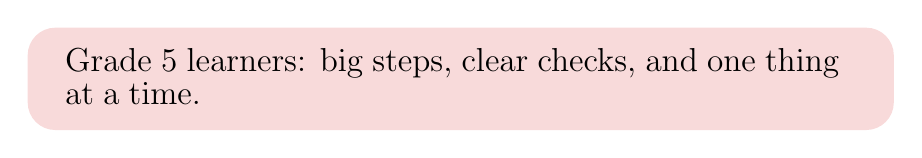
\begin{tikzpicture}
\fill[pbprimary!18, rounded corners=10pt] (0,0) rectangle (11,1.3);
\node[anchor=west, text width=10.2cm] at (0.35,0.68) {\large Grade 5 learners: big steps, clear checks, and one thing at a time.};
\end{tikzpicture}
\end{center}
\end{frame}
\begin{frame}{Todays Goal}
\begin{itemize}
\item I can explain current events that involve computing devices
\item I am aware of who has access to data in the digital spaces I am using
\end{itemize}
\begin{block}{Remember}
We do not have to be perfect right away. We take one step, then the next step, then we check.
\end{block}
\end{frame}
\begin{frame}{What You Need}
\begin{itemize}
\item Your class materials
\item The digital tool or build materials for today
\item A partner voice and your thinking
\end{itemize}
\begin{block}{Partner Norms}
Look. Listen. Try. Talk. Help without taking over.
\end{block}
\end{frame}
\begin{frame}{Step 1}
\begin{block}{Open the tool and follow the model slide.}
Open the tool and follow the model slide.
\end{block}
\begin{itemize}
\item Stay on the same screen as the class until the first example is complete.
\item Model the first screen and the exact tool students must use before release.
\end{itemize}
\centering\large\color{pbprimary} Pause. Check. Then move on.
\end{frame}
\begin{frame}{Step 2}
\begin{block}{Create your own content with the target feature.}
Create your own content with the target feature.
\end{block}
\begin{itemize}
\item Use the checklist so you know what must be included.
\item Provide a visible checklist so students know what counts as complete.
\end{itemize}
\centering\large\color{pbprimary} Pause. Check. Then move on.
\end{frame}
\begin{frame}{Step 3}
\begin{block}{Revise, save, and prepare to share.}
Revise, save, and prepare to share.
\end{block}
\begin{itemize}
\item Check that your work matches the success criteria before you turn it in.
\item Use sentence frames or model examples when students need help generating content, not just clicking tools.
\end{itemize}
\centering\large\color{pbprimary} Pause. Check. Then move on.
\end{frame}
\begin{frame}{If You Get Stuck}
\begin{enumerate}
\item Read the directions on your screen or slide one more time.
\item Check the example, the checklist, or your partner role.
\item Try one small change before asking for a full rescue.
\item Tool navigation can overshadow the content goal if too many options appear at once.
\end{enumerate}
\begin{alertblock}{Help Routine}
Stop. Breathe. Point to where you are stuck. Ask a specific question.
\end{alertblock}
\end{frame}
\begin{frame}{Show Your Learning}
\begin{itemize}
\item I stayed with the steps and used the help routine when I needed it.
\item I made, coded, explained, or revised something that matches the lesson goal.
\item I can point to one choice, fix, or idea I learned today.
\end{itemize}
\begin{block}{Before You Leave}
Save it, share it, explain it, or demonstrate it.
\end{block}
\end{frame}
\begin{frame}{Teacher Voiceover Cues}
\footnotesize
\begin{itemize}
\item Today we are working on current events in computing technology (creating an infographic in canva) day 2. Watch first, then try it with me.
\item If you feel stuck, stop at the checkpoint slide and use the help routine before you panic.
\item Show what you learned by saving, sharing, explaining, or demonstrating one clear success move.
\end{itemize}
\color{gray}This slide can be removed before student use if you only want the visual deck.
\end{frame}
\end{document}
